\section{Introduction}
\subsection{Community Structure Identification Problem}
The Community Structure Identification Problem (CSIP) is a foundational challenge in network analysis and graph theory. At its core, it grapples with the intricate task of unearthing the inherent groupings, or communities, within a network. 

These communities hold the essence of dense internal connections, where nodes readily interact and share information among themselves. Yet, their outward tendrils reach less frequently, creating distinct boundaries with other gatherings within the network.

In a nutshell, the CSIP is about finding hidden groups or cliques within a network. It's like discovering friend groups within a school or social circles in a town. 

These groups have tightly connected members but fewer ties to people outside their group.
This problem is crucial in many fields because it helps us understand how complex systems are organized and how they function. Some example: 
\begin{itemize}
\item\textbf{Social Networks: }Think about social networking sites like Facebook or Twitter. The challenge is to recognize unique clusters or communities of users who exhibit similar interests, share mutual social connections, or participate in comparable discussions. Identifying these communities enables the platform to understand user behavior better, tailor content suggestions, and identify influential users or potential communities of interest.
\item\textbf{Biological Networks:} Analyzing communities in protein-protein interaction networks can help us understand cellular functions and identify potential drug targets. For instance, finding tightly connected groups of proteins involved in a disease process could lead to new therapies.
\item\textbf{Online networks:} In online forums, discussion boards, or social media platforms, the Community Structure Identification Problem involves identifying clusters of users who interact and engage with each other on specific topics or interests. Uncovering these communities can help moderate online discussions, identify influential users, and facilitate content recommendation or targeted advertising.

\end{itemize}
Solving the Community Structure Identification Problem typically entails applying graph clustering algorithms to partition the network into cohesive communities. These algorithms are techniques that place individuals into their most likely friend groups. They often try to maximize modularity, which measures how well-defined the communities are. It's like checking if the friend groups make sense or if people are randomly scattered.
\begin{center}
\begin{figure}[!htp]
    \centering
    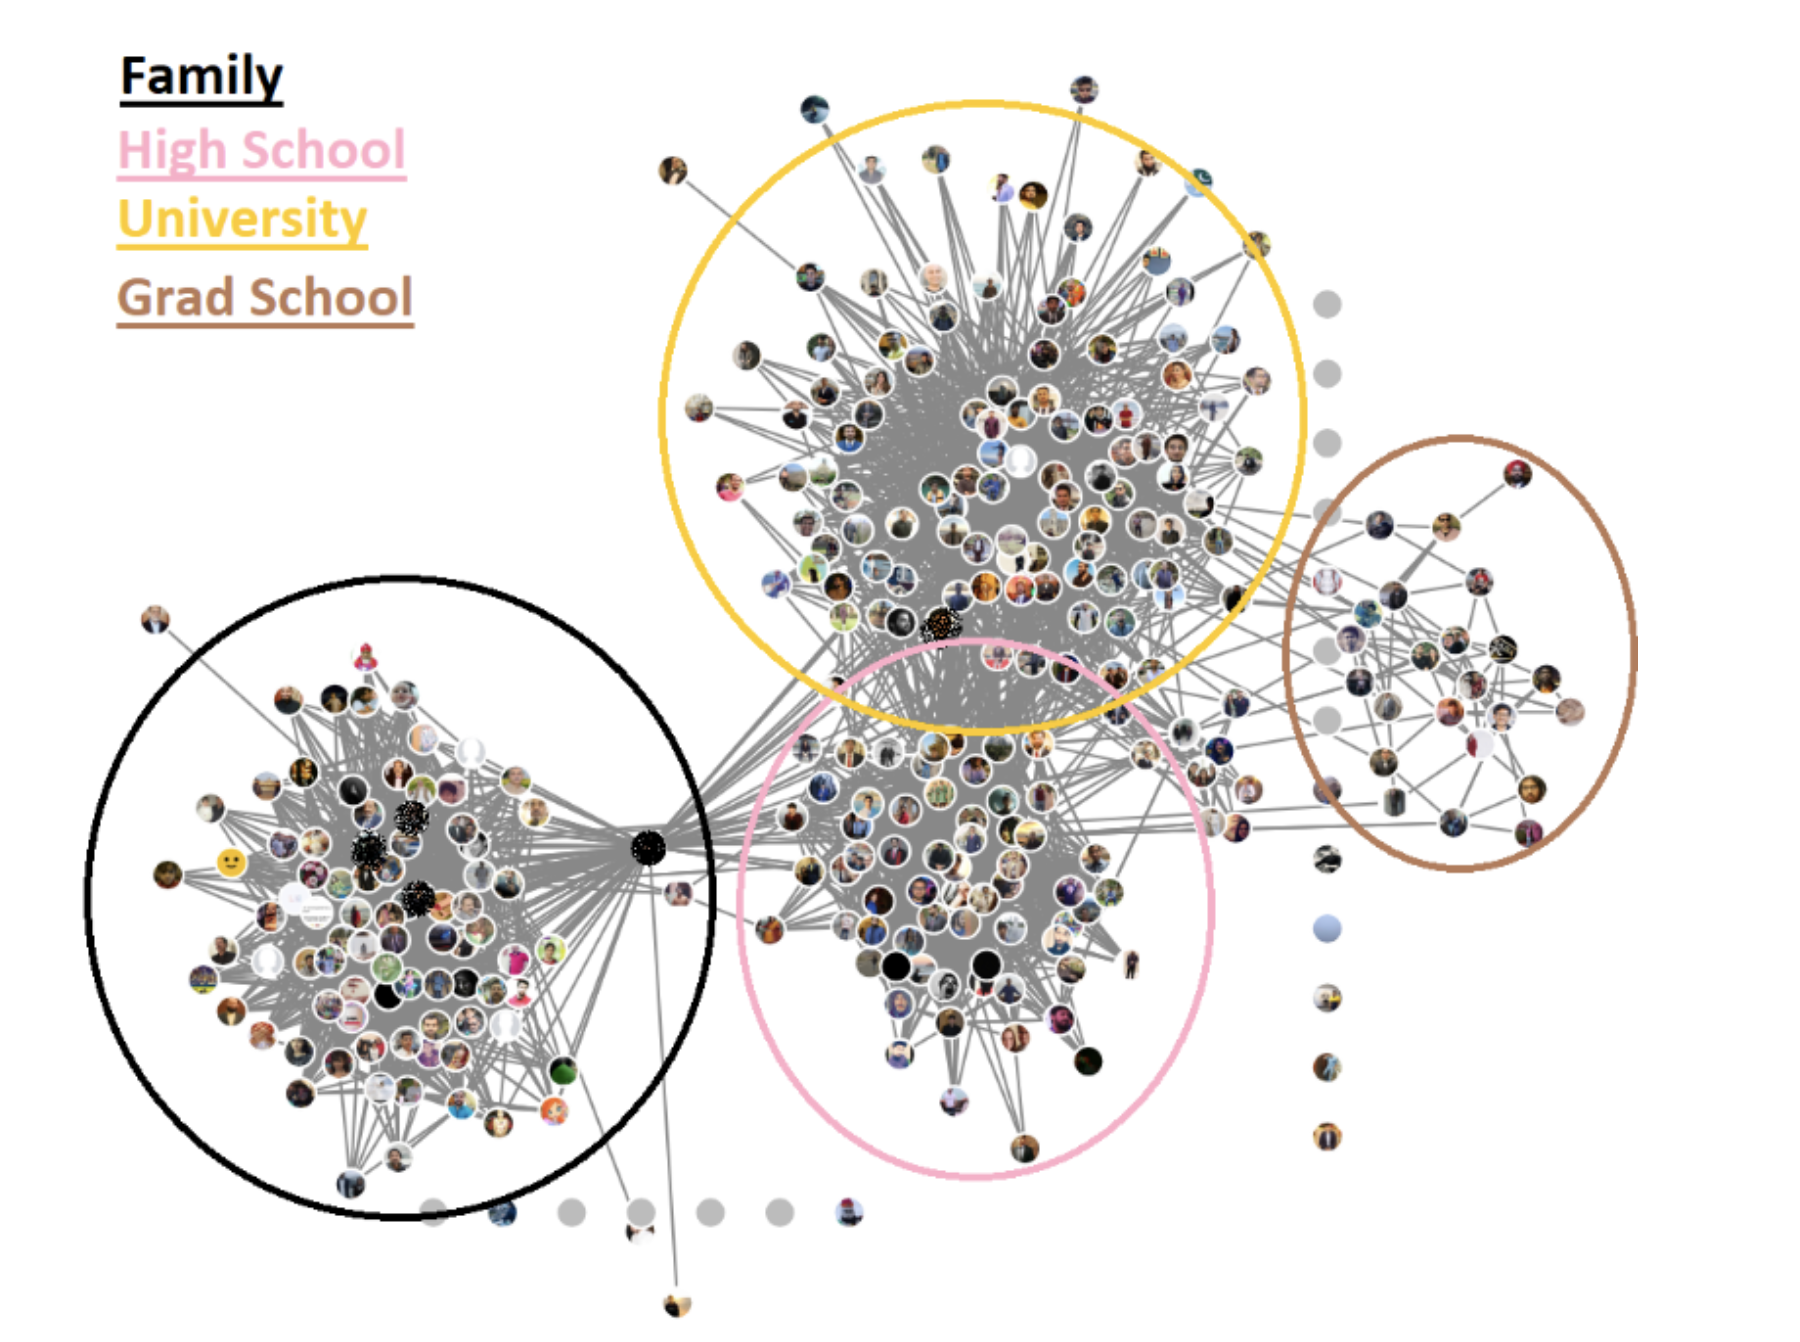
\includegraphics[width=0.8 \textwidth]{image/social_nx_example.png}
    \caption{Figure 1.1 Social Network Example}
    \label{subsection}
\end{figure}
\end{center}

\begin{figure}[!htp]
    \centering
    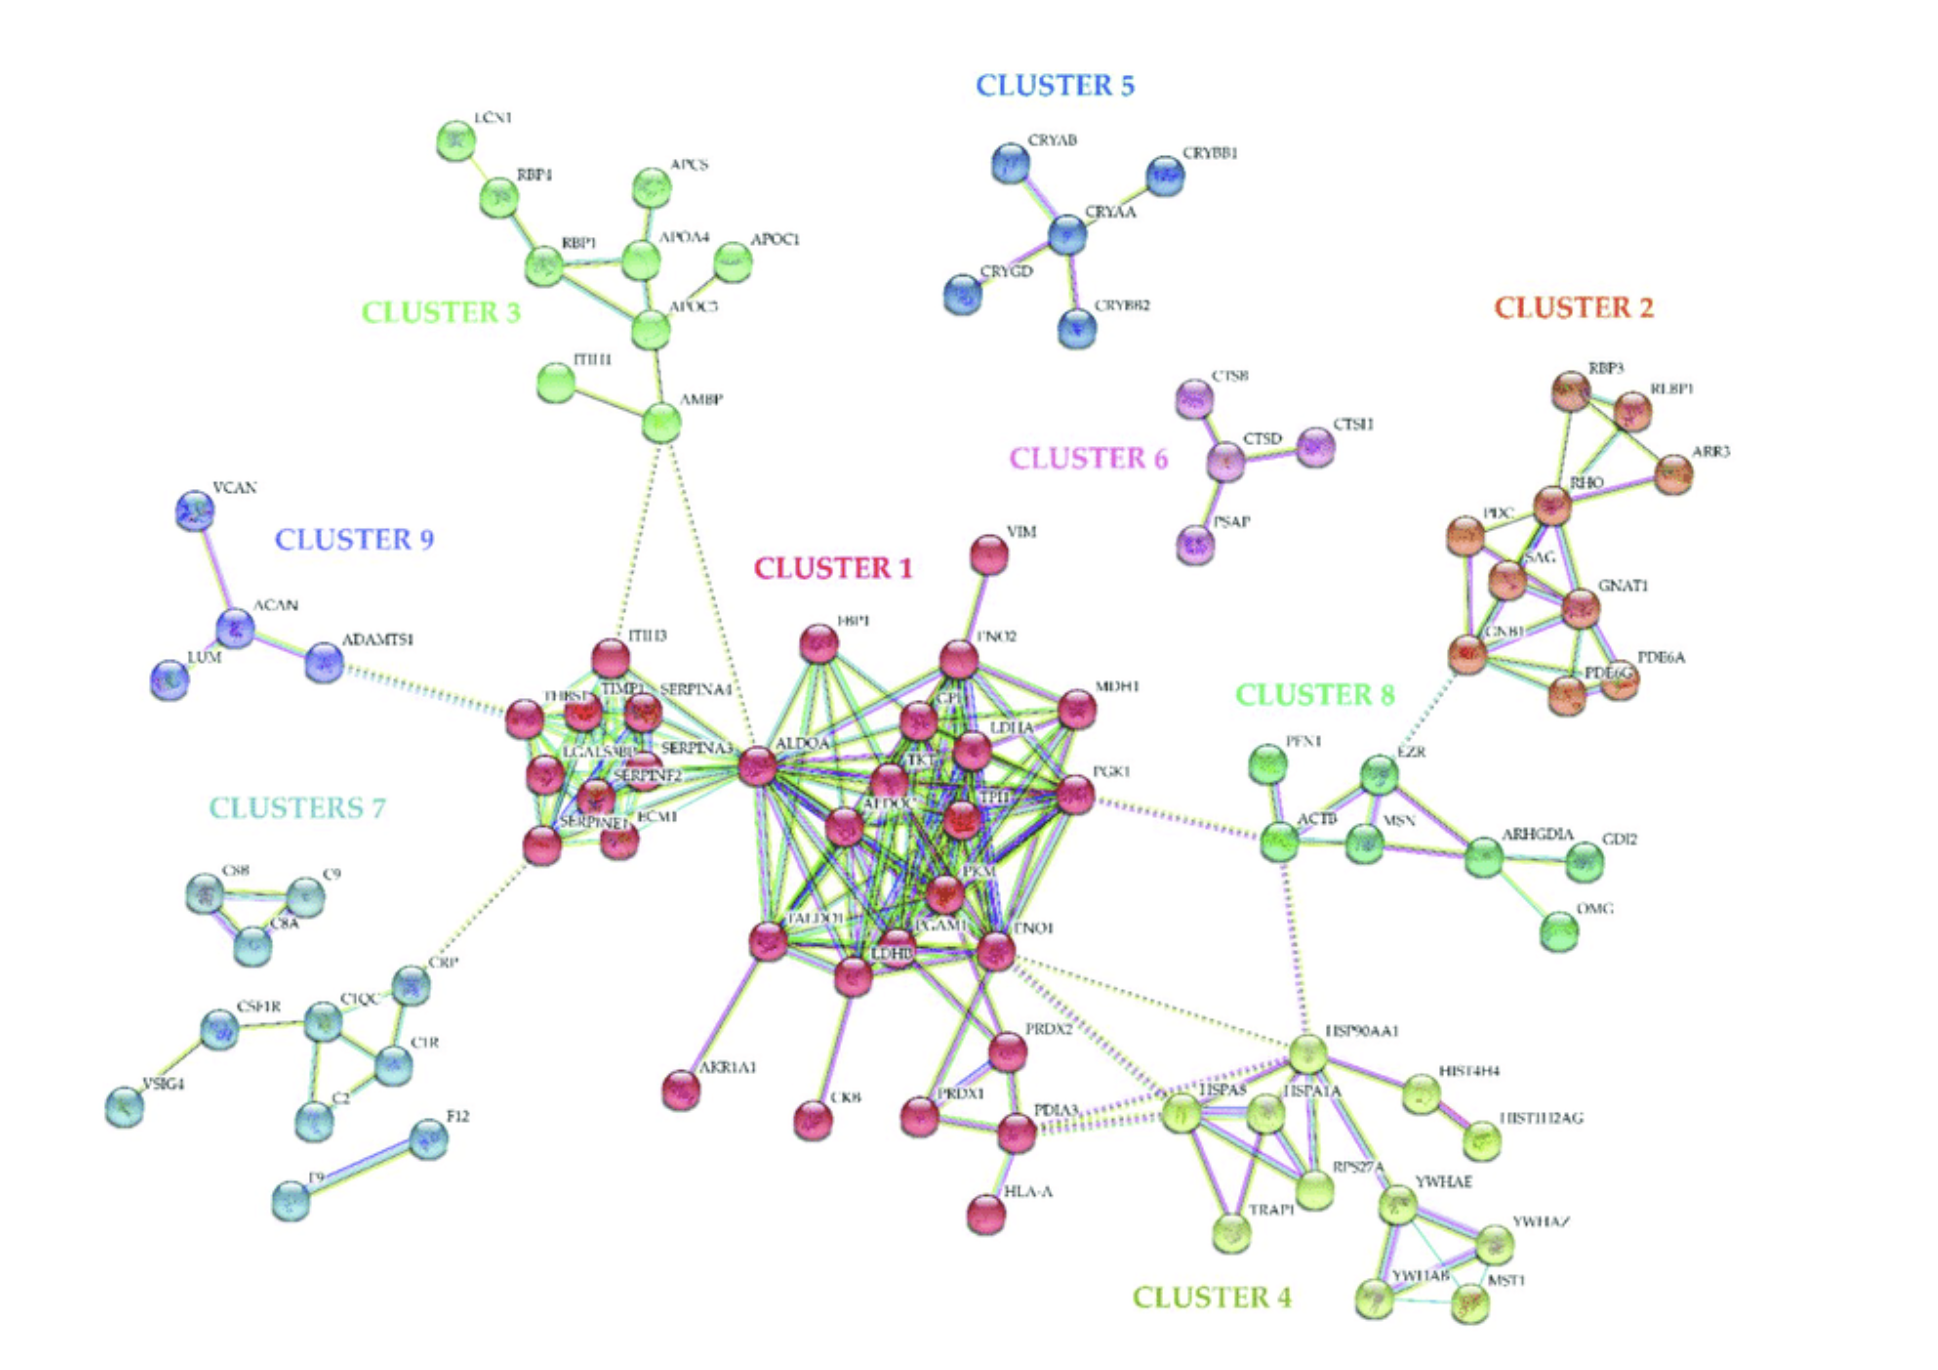
\includegraphics[width=0.8 \textwidth]{image/protein_interaction_example.png}
    \caption{Figure 1.2 Protein Interaction Network example
    }
    \label{subsection}
\end{figure}
\end{center}

\subsection{CSIP for user cluster and product rating}
\subsubsection{Motivation}
In the domain of E-commerce, characterized by a multitude of products vying for attention, the implementation of personalization emerges as a powerful strategy to transcend the noise. 
Imagine a digital storefront equipped with the ability to discern individual preferences even before user engagement, effectively directing customers towards products that evoke feelings of satisfaction and anticipation. 
This proposition is realized through the utilization of an application that harnesses the potential of user clustering and product rating prediction, thereby augmenting the overall shopping experience within this context.

By exploring the extensive collection of purchase histories and ratings, this technology uncovers interconnected communities of shoppers who share similar preferences and aspirations.
It can be likened to mapping the lively virtual marketplaces, revealing clusters where like-minded individuals gather around beloved brands, trending styles, or niche interests.

In this scenario, the Community Structure Identification Problem involves identifying clusters of users who share interests in product traits such as price, usability, maintainability, and brand,… and have bought similar products.
By uncovering these user communities, we can gain insights into the organization of the buying trends and identify groups of users related to interests, purchase characteristics, or needs.
\begin{center}
\begin{figure}[!htp]
    \centering
    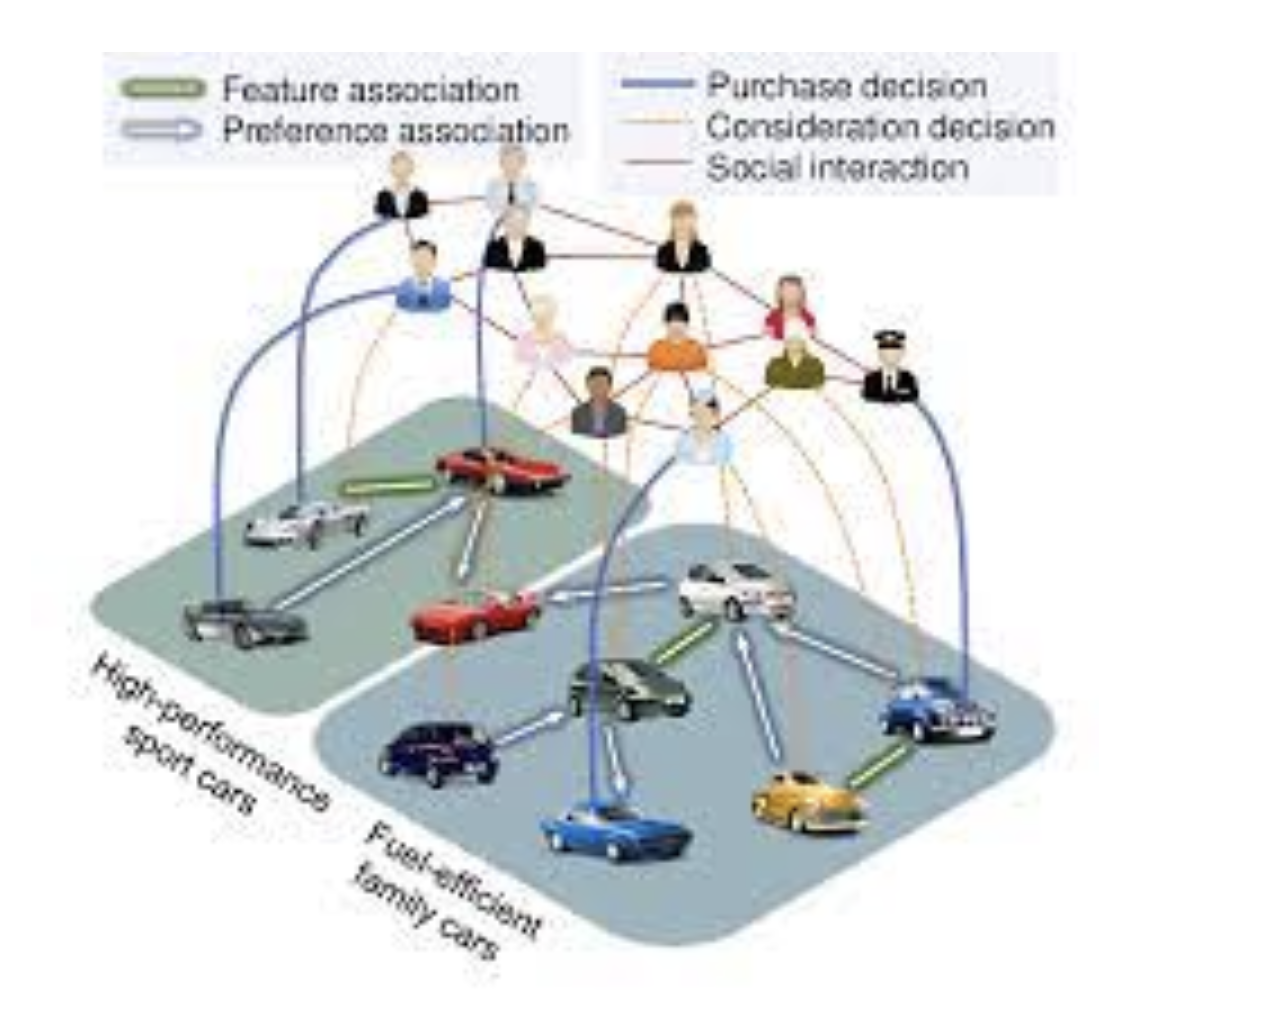
\includegraphics[width=1 \textwidth]{image/clustering_product_based.png}
    \caption{Figure 1.3 An example of how to cluster users based on product}
    \label{subsection}
\end{figure}
\end{center}\
For businesses, this insight unlocks a treasure trove of opportunities:

\begin{itemize}
    \item\textbf{Targeted Recommendations: }No more sifting through endless aisles. Each customer is greeted with a curated selection of products predicted to resonate with their unique preferences, fostering delight and satisfaction.
    \item\textbf{Personalized Discounts:}Promotions dance perfectly with individual desires, speaking to the heart of each cluster and igniting excitement for brands that truly understand their customers.
    \item\textbf{Strategic Product Development:} By analyzing the rating patterns of different clusters, businesses can uncover hidden gems, identify unmet needs, and tailor their product offerings to align with the evolving desires of their customers.
    \item\textbf{Dynamic Pricing:} Prices gracefully adjust to reflect the anticipated value of a product within a specific cluster, optimizing revenue while ensuring a sense of fairness and value for shoppers.
    
\end{itemize}
Beside, the benefits would extend beyond immediate sales, shaping a more meaningful and engaging customer experience:

\begin{itemize}
    \item\textbf{Relevant Content and Reviews: }Product descriptions and testimonials resonate more deeply when tailored to the interests of each cluster, fostering trust and connection.
    \item\textbf{Discovering New Delights:} Customers venture beyond their usual browsing habits, guided by recommendations that spark curiosity and introduce them to unexpected treasures they might have missed.
    \item\textbf{Building Brand Loyalty:} Personalized experiences cultivate a sense of belonging and appreciation, transforming customers into ardent advocates who eagerly share their positive experiences with others.
\end{itemize}
In summary, the Community Structure Identification Problem in the context of user clustering helps to reveal users with similar buying routines, combined with cluster average rating of a product to predict how a user who has never bought a product will rate it, enabling targeted marketing, recommendation systems, and a deeper understanding of market trend.

\subsubsection{Dataset and approach proposal}
\paragraph{Dataset}
\textbf{Context}: customer reviews and ratings of beauty-related products available on Amazon's platform.

\textbf{Content}: The dataset includes valuable information such as:
\begin{itemize}
    \item Unique User IDs for customer identification.
    \item Product ASIN (Amazon's distinctive product identifier).
    \item Ratings, which reflect customer satisfaction on a scale from 1 to 5.
    \item Timestamps, recorded in UNIX time, indicate when the ratings were submitted.
\end{itemize}
This dataset is just a fragment of the extensive Amazon product dataset, encompassing a staggering 142.8 million reviews spanning May 1996 to July 2014. 
The complete dataset provides a wealth of information, including detailed product reviews, metadata, category information, pricing data, brand details, and image features.
\paragraph{Approach proposal}
\begin{itemize}
    \item Step 1: involves constructing a user-user bipartite graph. Edges connect users who share a purchase history for the same product, representing potential affinities between them. This network serves as the foundation for subsequent community detection algorithms.
    \item Step 2: deploys clustering algorithms to partition the network into cohesive communities. These techniques leverage edge density and topological features to identify groups of users exhibiting stronger internal connections than external linkages.
    \item Step 3: Step into the realm of predictive modeling. Given a product and a user who has never purchased it, we leverage the power of their assigned community. By aggregating the average rating for that product among the user's community members, we generate an expected rating reflecting the collective sentiment of their peers. This effectively leverages shared preferences within the identified communities to infer potential individual behavior.
    \item Step 4: concludes the process with rigorous evaluation. We compare the predicted ratings with actual ratings garnered once the user purchases the product. Metrics like mean squared error or absolute error assess the accuracy of our community-based predictions, allowing us to refine our algorithms and improve prediction performance.
\end{itemize}
In summary, users are divided into groups based on common characteristics, such as similarity of rating patterns or similar demographic data. 
After that, the prediction of the rating of a user to an item is computed based on the opinions of other users in the same group

CSI presents a compelling application of network analysis and community detection in customer behavior modeling. By uncovering hidden communities and harnessing the power of shared preferences, we can effectively predict user ratings, personalize recommendations, and ultimately foster stronger customer relationships. This approach bridges the gap between individual interactions and collective behavior, revealing the hidden social fabric woven within large-scale online platforms.
